
\chapter{L'architecture calculateur} \label{CHAP3}
\smallskip
\hfill
\begin{minipage}[b]{8cm}
{\it Il est tr\`es important, pour celui qui souhaite d\'ecouvrir, de ne pas limiter son esprit \'a un seul chapitre de la
science mais plut\^ot de rester en contact avec plusieurs autres.}
\end{minipage}
\begin{flushright} Jacques Hadamard. \end{flushright}
\vskip 2cm


\section{Section Title}

\begin{tbd}
Commencer a pr\'esenter les diff\'erentes couches logiciel.\\

the following four stacks could become the basis for upcoming generations of cars in five to ten years:
\begin{itemize}

\item \emph{Time-driven stack}. In this domain, the controller is directly connected to a sensor or actuator while the systems have to support hard real-time requirements and low latency times; resource scheduling is time based. This stack includes systems that reach the highest Automotive Safety Integrity Level classes, such as the classical Automotive Open System Architecture (AUTOSAR) domain.
\item \emph{Event- and time-driven stack}. This hybrid stack combines high-performance safety applications, for example, by supporting ADAS and HAD capability. Applications and peripherals are separated by the operating system, while applications are scheduled on a time base. Inside an application, scheduling of resources can be based on time or priority. The operating environment ensures that safety-critical applications run on isolated containers with clear separation from other applications within the car. A current example is adaptive AUTOSAR.
\item \emph{Event-driven stack}.This stack centers on the infotainment system, which is not safety critical. The applications are clearly separated from the peripherals, and resources are scheduled using best-effort or event-based scheduling. The stack contains visible and highly used functions that allow the user to interact with the vehicle, such as Android, Automotive Grade Linux, GENIVI, and QNX.
\item \emph{Cloud-based (off-board) stack}. The final stack covers and coordinates access to car data and functions from outside the car. The stack is responsible for communication, as well as safety and security checks of applications (authentication), and it establishes a defined car interface, including remote diagnostics.
\end{itemize}

\url{https://www.mckinsey.com/industries/automotive-and-assembly/our-insights/rethinking-car-software-and-electronics-architecture}
\end{tbd}



\begin{figure}
    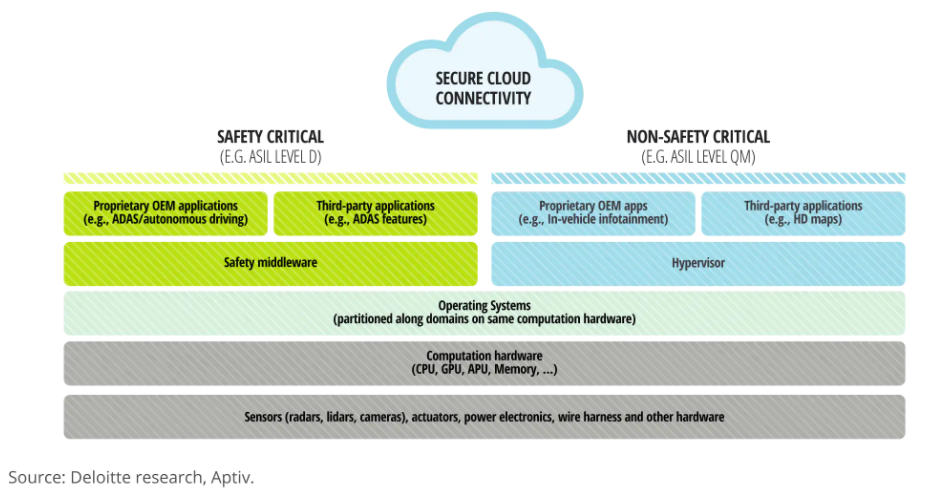
\includegraphics[width=\textwidth]{architecture}
    \caption{Architecture g\'en\'erique}
    \label{fig:archi}
\end{figure}
\url{https://www2.deloitte.com/us/en/insights/focus/future-of-mobility/pure-play-software-in-automotive-industry.html}
